\chapter{Thesis Evaluation}
\label{ch:evaluation}
This section provides the details of the experiments conducted on the system described in Chapter \ref{ch:contribution} and the analysis of the results. Two experiments are conducted on the system with a focus on obtaining information on the increase in the speed of the firmware update and efficiency of the system using uptime and downtime of the modules. The Digital Twin is used extensively for this purpose, as it displays the majority of the KPIs needed for this analysis.

\section{Experiment 1: Measurement of Simultaneous Firmware Update Efficiency}
\label{sec:exp1}
The \acrshort{SUIT} framework in RIOT OS allows the MCU to be updated using multiple methods such as Ethos, SLIP, and \acrshort{WiFi}. In this experiment, each module is initially updated through the network individually, by running the commands in the Linux terminal. These commands publish the updated firmware to the \acrshort{CoAP} fileserver and notify the module through the network interface about the new firmware to be installed. The process is elaborated through an Activity Diagram depicted in Figure \ref{fig:exp1}.

This experiment is performed both using a wired network connection with Ethos running over the serial link of the modules to the Linux host PC, and a wireless network connection (\acrshort{OTA}) using \acrshort{WiFi}. The results are very similar with regard to speed of update and hence are tabulated together.

\begin{figure}
    \centering
    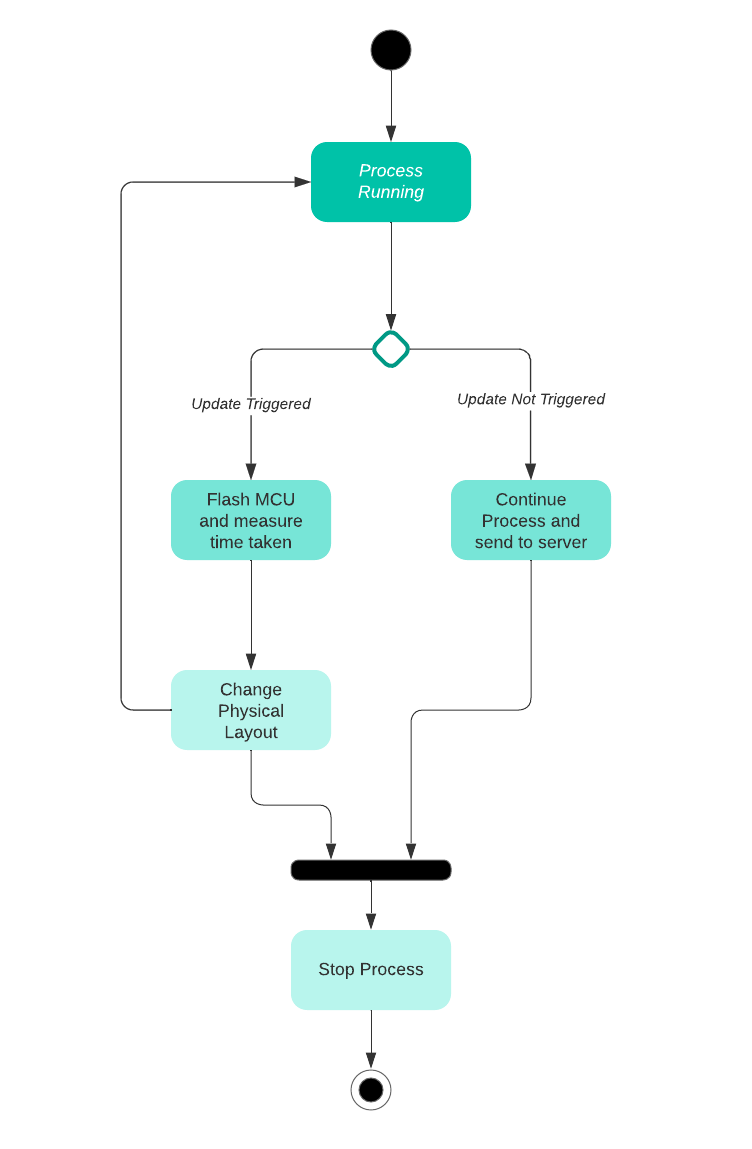
\includegraphics{images/Exp 1.png}
    \caption{Procedure for Experiment 1}
    \label{fig:exp1}
\end{figure}

Each module is updated individually for 50 iterations. The update time in seconds is measured and tabulated. Each individual module is then added to the network by adding a route from the interface to the network address. For the wireless network, the physical address of the module can be routed to the network. For the wired network, a TAP interface is created for each of the modules and a separate route is added from each module to the network through the TAP interface. All modules are updated simultaneously through the Digital Twin and the update time is measured and tabulated. The results for both tabulations are plotted as shown in Figure \ref{fig:updateTimes}.

\begin{figure}
    \centering
    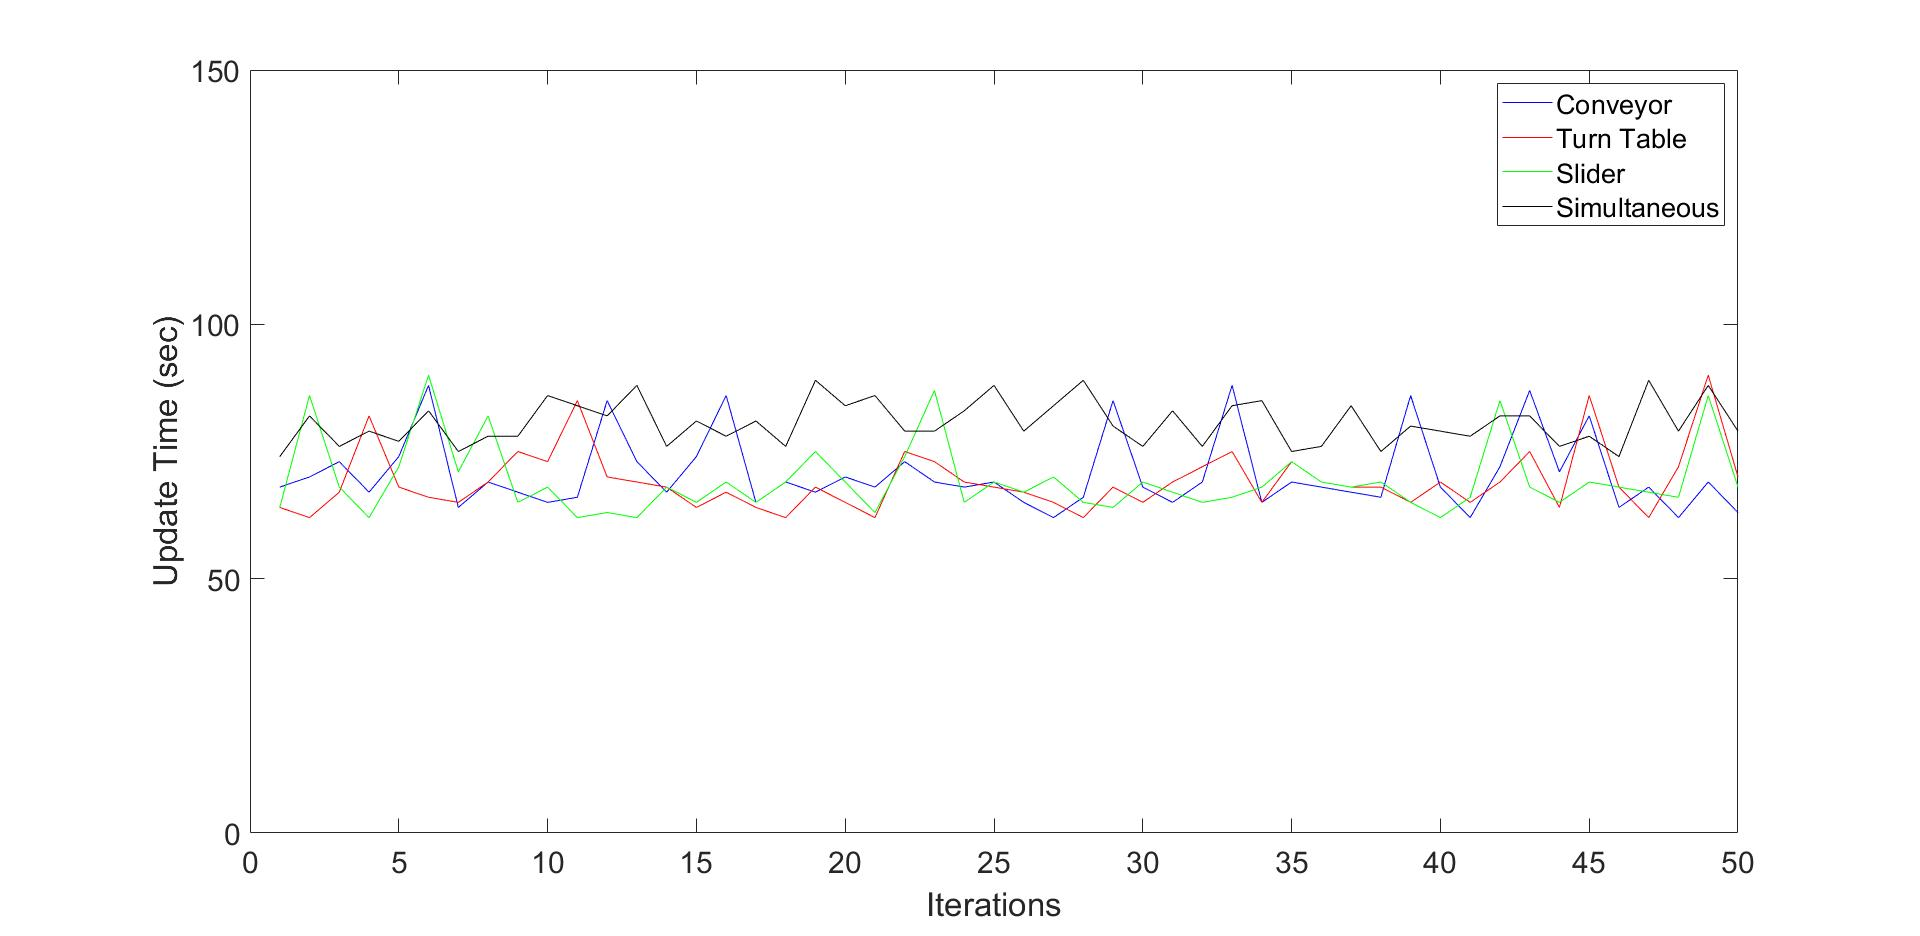
\includegraphics[scale=0.2]{images/UpdateTimes.jpg}
    \caption{Plot of Update Time for 50 Iterations}
    \label{fig:updateTimes}
\end{figure}

The average time taken for the firmware update of each individual module, measured as an average of 50 iterations, is displayed in Table \ref{tab:speed}. The total update time for both the individual module update and the simultaneous update is noted as shown in the equation below. Since there are 7 modules in each layout, the equation for individual updates adds the time taken for 4 conveyors, 2 turntables, and 1 slider.

\begin{table}[h!]
    \centering
\begin{tabular}{ | m{3cm} | m{2cm} | } 
  \hline
  \textbf{Module}&\textbf{Time\ (sec)} \\ 
  \hline
  Conveyor&70.62 \\ 
  \hline
  Turntable& 68.92 \\ 
  \hline
  Slider&69.22 \\
  \hline
\end{tabular}
    \caption{Factory Module Update Speeds}
    \label{tab:speed}
\end{table}

\begin{quote}
           \textit{Time Taken for all modules by individual update} $(t_{ind})$ =
       
       \textit{Sum of averages of update time for all modules} $(t_{ind\_avg})$

     \centering  $t_{ind}$ = $\sum(t_{ind\_avg})$

     \centering  $t_{ind}$ = $4\times conveyor + 2\times turntable + 1\times slider$
     
     \centering $t_{ind}$ = 489.54 sec
     
     \textit{Time Taken for all modules by simultaneous update} ($t_{sim}$) = \textit{Average of update time for simultaneous update} ($t_{sim\_avg}$)
    
     $t_{sim}$ = 80.64 sec
     
     \textit{Increase in update speed due to simultaneous update } = 
     \dfrac{t_{ind}}{t_{sim}}
     
     \textit{Increase in update speed = \dfrac{489.54}{80.64} }
     
     \textit{Increase in update speed = 6.07}
\end{quote}

The results show that the simultaneous firmware update leads to a 6.07 times increase in update speed, while also proving that the simultaneous update speed increases proportionally with the increase in the number of factory modules added to the layout.

\section{Experiment 2: Measurement of System Efficiency}
The Digital Twin displays the Uptime of each factory module when it is in motion and the total running time of the entire system which can used to calculate the process efficiency of the system. This experiment is conducted by running the system continuously for 30 minutes, with each workpiece being transported individually. Each workpiece is produced as soon as its predecessor is dispatched to emulate continuous processing. The working procedure is depicted in the activity diagram in Figure \ref{fig:exp2}.

\begin{figure}
    \centering
    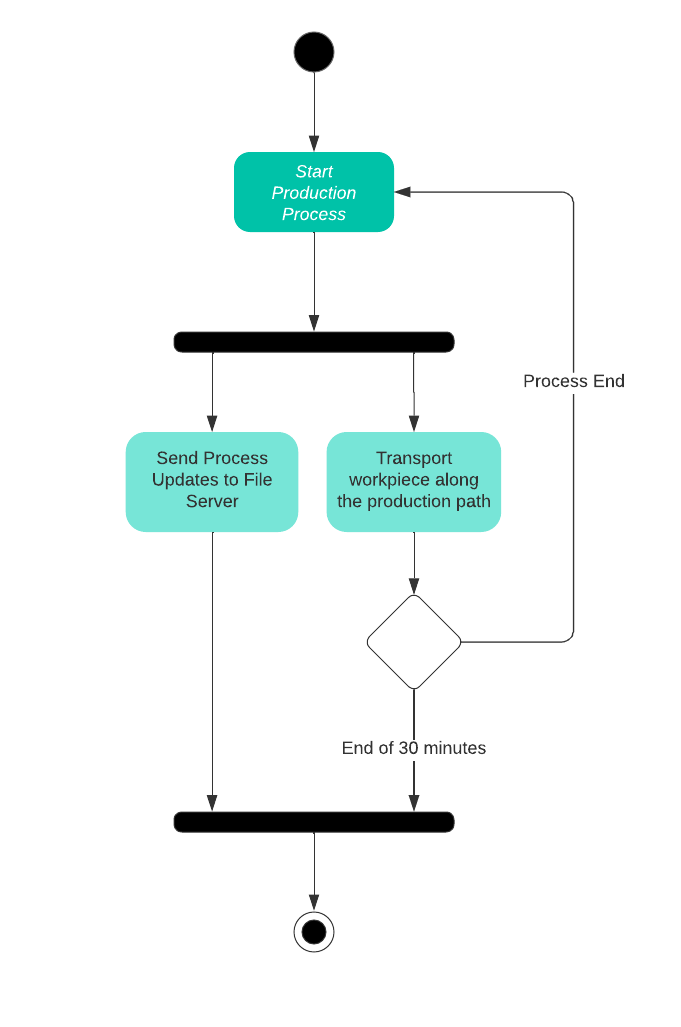
\includegraphics{images/Exp2.png}
    \caption{Procedure for Experiment 2}
    \label{fig:exp2}
\end{figure}

The uptime of all the modules after 30 minutes of running the process can be observed in the Digital Twin as shown in Figure \ref{fig:runtime}. The timings are tabulated in Table \ref{tab:efficiency}.

\begin{figure}
    \centering
    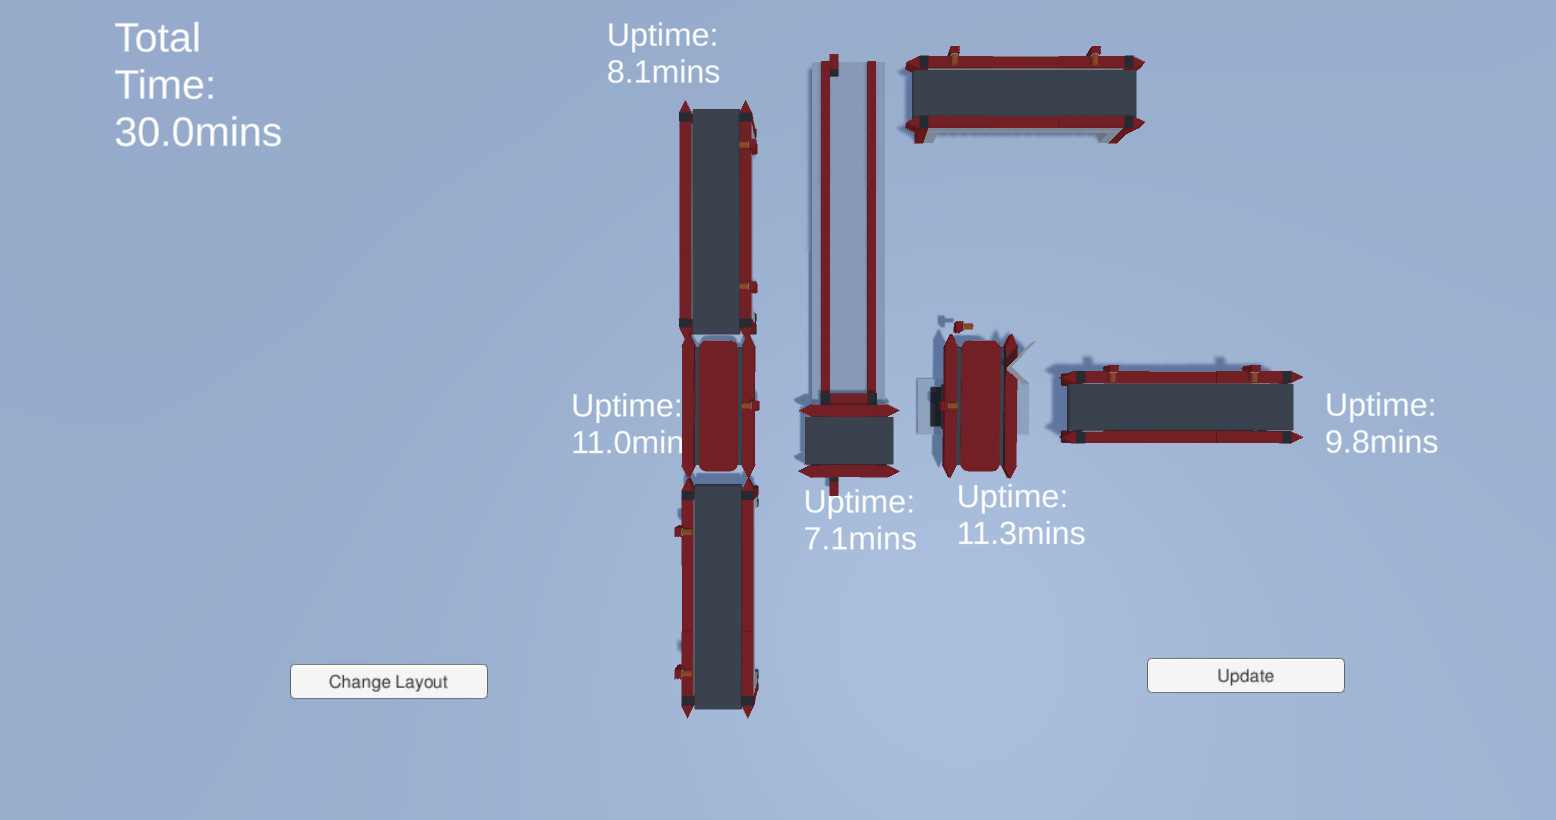
\includegraphics[scale=0.35]{images/Runtimes.png}
    \caption{Runtime of individual modules}
    \label{fig:runtime}
\end{figure}

\begin{table}[h!]
    \centering
\begin{tabular}{ | m{4cm} | m{2cm} | } 
  \hline
  \textbf{Module}&\textbf{Time\ (min)} \\ 
  \hline
  Production Conveyor&8.1 \\ 
  \hline
  Production Turntable& 11.0 \\ 
  \hline
  Slider&7.1 \\
  \hline
  Dispatch Turntable&11.3 \\
  \hline
  Dispatch Conveyor&9.8 \\
  \hline
  Total Running Time&30.0 \\
  \hline
\end{tabular}
    \caption{Runtime of modules and total time}
    \label{tab:efficiency}
\end{table}

The total time taken by the workpiece to be transported from production to dispatch is called Cycle Time. The measured Cycle Time of the system can be calculated by the sum of the runtime of all involved modules in the process. The ideal Cycle Time of the system, when the system runs at 100\% efficiency, is the total runtime of the system displayed in the Digital Twin. The efficiency of the system can be measured using these values as shown in the equations below.

\begin{quote}
    \textit{Measured Cycle Time of the System ($t_{sum}$) = 47.3 mins}
    
    \textit{Ideal Cycle Time of the System ($t_{ideal}$) = 30 mins}

    \textit{System Efficiency = $\dfrac{t_{ideal}}{t_{sum}}$ $\times 100}$

    \textit{System Efficiency = \dfrac{30}{47}\times100}
    
    \textit{System Efficiency = 63.42\%}
\end{quote}
%\todo[]{Graph of total time vs. individual module time}

The efficiency of the system for the experimented layout (Layout 1) is calculated to be 63.42\%. The moderate efficiency can be attributed to multiple factors such as the offset of the sensor placement on the modules and increased usage of the hardware over several years resulting in decreased motion speed of the factory modules. The efficiency can be improved by methods such as increasing the power input to the modules and conducting regular hardware maintenance or replacement.

% \section{Experiment 3: Measurement of OTA Update Success Rate}
% As mentioned previously, the wireless network connectivity at OvGU does not provide IPv6 addresses to its connected nodes. This experiment was performed using a home network that provided IPv6 addresses which enabled the firmware update process to be performed over WiFi.

% The process is similar to Experiment 1 (Section \ref{sec:exp1}) where the update is performed using SUIT framework, but since the experiment is performed outside the university, only a single module is connected to the network and the update time is measured.

These experiments provide conclusive proof of the feasibility of developing such a system and its advantages in the context of manufacturing processes. Experiment 1 proves the efficiency of the simultaneous firmware updates by comparing individual module update time to simultaneous update time. In Experiment 2, the workload of each module is measured and efficiency is calculated which is useful to find out which modules are being overused or unused, and can be used to avoid bottlenecks and calculate potential alternatives for production paths. 
% Experiment 3 displays the risks of using wireless OTA updates by measuring the OTA update success rate.